\section{Realization of the Bott cancellation in the reduced algebra}
\label{sec:assembly}

We now prove that the rank-zero Bott class of the embedded torus
$\langle z,x\rangle$ vanishes in the reduced group algebras along a tail
of the compatible accuracy sequence constructed below.  The localized Bott
profiles from Section~\ref{sec:analysis} can be moved between neighboring heights.
We realize two families of these moves by finite Cayley formulas, using
the disjoint domains of Proposition~\ref{prop:domains}.  As the errors
tend to zero, the formulas give exact projection homotopies in a norm
sequence quotient.  Their cancellation removes the initial-height
profile.  We then identify that profile with the physical torus Bott
class and recover an exact finite witness in a single reduced group
algebra, before passing to a finitely generated subgroup.

We use the right Cayley graph and the conventions of
Proposition~\ref{prop:graphical-realization}.  Thus a positive formal edge is
$g\longrightarrow g\sigma$, the deck group acts on the left, and, after
choosing one lift of each base vertex $v$, the embedded cover has coordinates
\begin{equation}\label{eq:assembly-cover-coordinates}
 j(v,f)=f t_v\qquad(f\in\HH).
\end{equation}
We identify $\HH$ with its embedded image in $\Gamma$.  Its distinct sheets
are the left translates $h\widetilde X$, indexed by the cosets $h\HH$.
On $\ell^2(\Gamma)$ put
\[
 R(g)\delta_h=\delta_{hg^{-1}}.
\]
This is the right regular representation with the convention that
$R(g)R(k)=R(gk)$.  The unitary $I\delta_h=\delta_{h^{-1}}$ satisfies
\begin{equation}\label{eq:right-left-regular}
 I R(g) I=\lambda(g).
\end{equation}
Consequently the norm closure of the right regular group algebra is a copy
of $\Cr(\Gamma)$.  We use it throughout the estimates and apply
\eqref{eq:right-left-regular} at the end.  This equivalence sends the represented
group element $g$ to the same element $g$, so it does not introduce an
antihomomorphism on group $K$-theory.
We orient each positive old incidence edge from its $\mathscr A$ endpoint
$v$ to its $\mathscr B$ endpoint $w$.  If its label is $\sigma$ and its
forward voltage is $h_e$, then
\begin{equation}\label{eq:assembly-edge-direction}
 t_v\sigma=h_e t_w,
 \qquad
 R(\sigma)\delta_{f t_w}=\delta_{f h_e^{-1}t_v}.
\end{equation}
Thus the $\mathscr B$-to-$\mathscr A$ incidence block of $R(\sigma)$ is
the deck operator $R_{\HH}(h_e)$.  For our chosen direction a sampled
term $R_{\HH}(v_e)$ is implemented by the forward voltage $h_e=v_e$.
The opposite, forward transition operator has the adjoint convention.

We will take a sequence of constructions, indexed by $\nu$.  The integer $b$
is fixed once, including across this sequence.  The parameters $s=s_\nu$ and
$H_0=H_{0,\nu}$ may increase; the degree is fixed at all heights of any one
construction.  All matrix sizes in the Bott representatives below are fixed.
The number of incidence types, the finite weight net, and the lengths of
operator products may depend on $\nu$; these choices precede the choice of
$s_\nu$.

\subsection{Compact Bott profiles and common carriers}

Use throughout the compact Bott projection $p$ in
Equation~\eqref{eq:compact-bott-profile}, with $m=2$,
$e=e_\infty=\operatorname{diag}(0,1)$, and $a=p-e$.
The explicit eigenvectors and winding calculation in
Section~\ref{sec:analysis} prove that $[p]-[e]$ is a compactly supported
Bott generator.  This projection and its signed class are fixed for the
entire accuracy sequence.

In angular torus coordinates $(\zeta,\xi)\in(\R/\Z)^2$ corresponding to
$(z,x)$, put
\[
 Z_i=2^{500H_i},\qquad N_i^{\mathrm{freq}}=2^{200H_i},\qquad J_i=2^{50H_i},
 \qquad
 a_i(\zeta,\xi)=a\bigl(Z_i(\zeta-\alpha),N_i^{\mathrm{freq}}\xi\bigr).
\]
The functions are defined in a small coordinate chart and extended by zero;
their supports lie strictly inside that chart.  Thus $e+a_i$ is a smooth
projection on the torus.  It has the same first Chern number as $p$, so
\begin{equation}\label{eq:physical-bott-profile}
 [e+a_i]-[e]=\beta\quad\hbox{in }K_0(C(\mathbb T^2)),
\end{equation}
where $\beta$ is the torus realization of this fixed rank-zero Bott
generator.  The positive rescalings preserve its sign.

The rescaling path
\begin{equation}\label{eq:adjacent-rescaling}
 a_{i,t}(\zeta,\xi)
 =a\bigl(2^{500bt}Z_i(\zeta-\alpha),
          2^{200bt}N_i^{\mathrm{freq}}\xi\bigr),\qquad 0\le t\le1,
\end{equation}
joins $a_i$ to $a_{i+1}$.  Each $e+a_{i,t}$ is a projection.  In the rescaled
coordinates all these functions form one compact smooth family.  In
particular there is a common modulus of norm continuity in $t$, independent
of $i$ and $\nu$, because $b$ is fixed.

Choose real continuous smooth cutoffs $\chi_i$, with $0\le\chi_i\le1$,
equal to one on the supports of all profiles used at level $i$, including the
profiles $a_{i-1,t}$ transported from the preceding level.  Their supports
are contained in fixed enlargements, depending only on $b$, of the rectangle
at level $i$.  Choose an additional slightly larger Borel rectangle projection
$e_i^{\mathrm{car}}$ containing $\supp\chi_i$.  We use the same choices on
both sides of a layer.  They may be chosen so that every function used in a
block $(i,k)$, $|i-k|\le1$, is supported where both $\chi_i$ and $\chi_k$
equal one.  Indeed the largest required support at level $i$ is contained in
the rectangle of level $i-1$, and the ratios between successive widths are
the fixed numbers $2^{500b}$ and $2^{200b}$.  At $i=0$ the notation $i-1$
merely prescribes a fixed enlargement, not an additional graph layer.

Apply Proposition~\ref{prop:sampled-symbols} with these fixed enlargements.
The spread operators from Lemma~\ref{lem:supported-spreading}, written
in the right regular representation, have the form
\[
 T_i=\sum_j a_{ij}R(y)^j,
 \qquad \sum_j|a_{ij}|^2=1,
 \qquad e_i^{\mathrm{car}}T_i^*T_i e_i^{\mathrm{car}}
       =e_i^{\mathrm{car}}.
\]
Their range carriers
\begin{equation}\label{eq:spread-carrier}
 P_i=T_i e_i^{\mathrm{car}}T_i^*
\end{equation}
are projections in the containing von Neumann algebra and satisfy
\begin{equation}\label{eq:carrier-trace}
 \tau_{\HH}(P_i)=\tau_{\HH}(e_i^{\mathrm{car}})
       \le C_{\nu}2^{-700H_i}.
\end{equation}
The constant is uniform in the height.  Increasing the starting height
ensures the disjointness of the translates even for the specified enlarged
rectangles.  These Borel carriers are used only for Hilbert-space estimates.
Actual group-algebra formulas below use continuous functions and the finite
sums $T_i$; no Borel carrier is asserted to belong to a reduced $C^*$-algebra.

For one construction put $\mathscr L=\ell^2(\Gamma)$ and regard
$e_i^{\mathrm{car}}$ as a projection on $\mathscr L$ through the subgroup's
right regular operators.  The model space is
\begin{equation}\label{eq:exact-model-space}
 \mathscr K=\bigoplus_{i\ge0}e_i^{\mathrm{car}}\mathscr L.
\end{equation}
A band profile $f=(f_{ik})_{|i-k|\le1}$ from our fixed compact profile
families acts on this space from the $k$th to the $i$th summand by its
torus function $f_{ik}$.  Support in both carriers makes each block
well defined; the uniform block norm and width one give a bounded
operator $f^{\mathrm{mod}}$.
All cosets of $\HH$ carry the same profile.

The profiles we must realize have the four diagonal height patterns
\[
 \begin{array}{c|ccccc}
  &0&1&2&3&\cdots\\ \hline
  \mathrm{ev}&a_0&0&a_2&0&\cdots\\
  \mathrm{od}&0&a_1&0&a_3&\cdots\\
  \mathrm{ev},+&0&0&a_2&0&\cdots\\
  0&a_0&0&0&0&\cdots
 \end{array}
\]
Each entry is a compactly supported difference from the common scalar
projection $e$; a zero entry retains that scalar part in the full projection.  Rotating
between the disjoint pairs $(0,1),(2,3),\ldots$ and then applying
\eqref{eq:adjacent-rescaling} moves the even pattern to the odd pattern.
The pairs $(1,2),(3,4),\ldots$ similarly move the odd pattern to the
positive-even pattern.  The even pattern also splits into the
initial-height and positive-even patterns.  Our analytic task is to
realize these four profiles and the two paths in one fixed matrix size.
The estimates below first pass from this model to normalized constants
on the sheets, and then from the sheets to finite Cayley formulas.

\subsection{Domains, trimming, and bounded maps}

For this subsection fix one construction.  Let
\[
 \mathscr H_{\mathrm{abs}}=\bigoplus_Q\ell^2(Q)
\]
be the abstract orthogonal sum over its sheets.  A fixed finite matrix factor
can be tensored onto every space without changing the argument.  On each
old vertex of height $i$ use the carrier $P_i$ of
\eqref{eq:spread-carrier}.  More precisely, using the regular deck coordinate
on the lifted vertex set, let $E_{Q,i}$ be the sum of these carriers over the
old base vertices on both sides of height $i$ in sheet $Q$.  Put
\[
 E_i=\bigoplus_Q E_{Q,i},\qquad E=\bigoplus_{i\ge0}E_i.
\]
All these projections are zero on private-vertex coordinates.

Let $D_Q$ be the domains from Proposition~\ref{prop:domains}, and let $D$ be
coordinate restriction to their abstract sum.  Their physical images are
pairwise vertex-disjoint.  Thus coordinate inclusion defines a partial
isometry
\[
 U\colon\mathscr H_{\mathrm{abs}}\longrightarrow\ell^2(\Gamma),
 \qquad U^*U=D,
\]
which is an isometry on $D\mathscr H_{\mathrm{abs}}$ and is zero on its
orthogonal complement.

\begin{lemma}[Uniform trimming estimate]\label{lem:assembly-trimming}
For a construction whose constants have already been fixed,
\[
 \|(1-D_Q)E_{Q,i}\|^2\le C_\nu2^{-690H_i},
 \qquad
 \delta_\nu:=\|(1-D)E\|\le C_\nu2^{-345H_0}.
\]
In particular $H_{0,\nu}$ can be chosen so that $\delta_\nu\to0$.
If $A=EAE$ and $B=EBE$, and
\[
 \Psi_\nu(A)=UDADU^*,
\]
then
\begin{equation}\label{eq:domain-product-error}
 \|\Psi_\nu(A)\Psi_\nu(B)-\Psi_\nu(AB)\|
       \le\delta_\nu^2\|A\|\|B\|.
\end{equation}
\end{lemma}

\begin{proof}
For a projection $P$ and a finite coordinate set $B_0$, the ordinary
Hilbert--Schmidt norm gives
\[
 \|1_{B_0}P\|^2\le\|1_{B_0}P\|_{\mathrm{HS}}^2
       =\sum_{u\in B_0}\langle P\delta_u,\delta_u\rangle.
\]
In a matrix amplification one sums over the fixed matrix basis as well.
Every regular deck translate of a given old vertex has the same diagonal
trace.  If the removed set in $Q$ is an old-centered ball, then
Proposition~\ref{prop:domains} bounds its entire cardinality by $2^{10H_i}$
whenever it meets height $i$.  Equation~\eqref{eq:carrier-trace} therefore
gives the first estimate, with all repeated deck lifts counted separately.
An empty removed set costs nothing.  A private singleton also costs nothing,
since $E_{Q,i}$ has zero private coordinates.  This statement is about indexed
sheet coordinates even if the same physical vertex is old in another sheet.

Both $D$ and $E$ preserve the height decomposition.  The norm of their
orthogonal direct sum is the supremum of the block norms, which gives the
bound on $\delta_\nu$.  Finally, using $U^*U=D$, the difference in
\eqref{eq:domain-product-error} is $UD A(D-1)B D U^*$.  Its norm is at most
$\|A\|\|B\|\,\|E(1-D)E\|$, and
$\|E(1-D)E\|=\|(1-D)E\|^2$.
\end{proof}

Trimming gives the almost multiplicative map needed for all model
profiles.  To compare the initial-height profile with the physical torus
class, we also need to sum its normalized constants over sheets.  Let
$\mathcal J$ initially sum finitely supported vectors from finitely many
abstract sheets into their physical vertex coordinates.  This notation does
not presume that untrimmed summation is bounded.

\begin{lemma}[Synthesis on the active carriers]\label{lem:assembly-synthesis}
Let $n_i$ be the number of surviving old base vertices on both sides of height
$i$.  Then
\begin{equation}\label{eq:raw-synthesis-level}
 \|\mathcal J(1-D)E_i\|^2
 \le n_i\sup_Q\|(1-D_Q)E_{Q,i}\|^2
 \le C_\nu2^{-689H_i}.
\end{equation}
Consequently $\mathcal J E$ extends to a bounded operator and
\begin{equation}\label{eq:raw-synthesis-sum}
 \|\mathcal J E-UDE\|
 \le C_\nu\sum_{i\ge0}2^{-344.5H_i}
 =C_\nu\frac{2^{-344.5H_0}}{1-2^{-344.5b}}.
\end{equation}
\end{lemma}

\begin{proof}
For a physical vertex $u$ and a specified old base vertex $v$, the only sheet
coset that can contain $u$ at base type $v$ is
$u t_v^{-1}\HH$, by \eqref{eq:assembly-cover-coordinates}.  This also follows
from the incidence bijection in Lemma~\ref{lem:sheet-incidences}.  Thus at
height $i$ each physical vertex receives at most $n_i$ indexed coordinates.
Pointwise Cauchy--Schwarz gives the first inequality in
\eqref{eq:raw-synthesis-level}, initially on the stated dense domain.
The layer cardinalities give
$n_i\le C_s2^{H_i}$; Lemma~\ref{lem:assembly-trimming} gives the second
inequality.  The bounded extensions at individual heights may be summed in
operator norm, because $H_i=H_0+bi$ and the square-root estimates are
summable.  On their common dense domain
$\mathcal J E=UDE+\mathcal J(1-D)E$, proving
\eqref{eq:raw-synthesis-sum} and the claimed extension.
\end{proof}

\subsection{Finite Cayley formulas and extraction of constants}

The incidences supplied by Propositions~\ref{prop:tower-labels},
\ref{prop:sequential-law}, and~\ref{prop:pruning} will be denoted by
$U_{ik}^0\colon\ell^2(\mathscr B_k)\to
\ell^2(\mathscr A_i)$ for a pre-deletion normalized incidence,
$|i-k|\le1$, suppressing its finite type index.  It sends the normalized
constant vector to the normalized
constant vector, its adjoint does the same, and its centered norm is at most
the fixed $\rho<1$.  Let $U_{ik}$ be its compression to the surviving vertex
sets.  The deletion fraction is at most $\varepsilon_{\mathrm{del}}$ in
each side and layer.  We always normalize constant vectors using the actual
surviving vertex counts.

\begin{lemma}[Deleting a small fraction of vertices]\label{lem:deleted-incidence}
There are contractions $\widehat U_{ik}$ on the surviving spaces that send
normalized constants exactly to normalized constants in both directions,
have centered norm at most $\rho$, and satisfy
\[
 \|U_{ik}-\widehat U_{ik}\|\le C\sqrt{\varepsilon_{\mathrm{del}}}.
\]
The constant is uniform in the height and the incidence type.
\end{lemma}

\begin{proof}
For one incidence let $a,b$ be the old normalized constants and let $P_A,P_B$
be the surviving coordinate projections.  Their normalized restrictions
$a',b'$ differ from $a,b$, after extension by zero, by at most
$C\sqrt{\varepsilon_{\mathrm{del}}}$.  Put
$Q_A=1-|a'\rangle\langle a'|$ and
$Q_B=1-|b'\rangle\langle b'|$ on the surviving spaces and define
\[
 \widehat U=|a'\rangle\langle b'|+Q_AUQ_B.
\]
Write $U^0=|a\rangle\langle b|+U_0$.  Then
$Q_AP_Aa=0$ and $Q_BP_Bb=0$, so $\|Q_AUQ_B\|\le\|U_0\|\le\rho$.
The two displayed summands of $\widehat U$ have orthogonal source and range
spaces, proving its asserted gap and norm.  The estimates
$\|Ub'-a'\|+\|U^*a'-b'\|\le C\sqrt{\varepsilon_{\mathrm{del}}}$
bound the remaining three blocks in $U-\widehat U$.
\end{proof}

We embed the model space \eqref{eq:exact-model-space} using normalized
constants on the surviving $\mathscr B_i$ vertices.  The subgroup operators
preserve $\mathscr L=\bigoplus_{h\HH}\ell^2(h\HH)$.  For each coset and
height, map its vector to the corresponding sheet's normalized constant
array, applying $T_i$ to its deck coordinate.  This defines an isometry
\[
 \mathcal I\colon\mathscr K\longrightarrow\mathscr H_{\mathrm{abs}},
 \qquad \mathcal I\mathcal I^*\le E.
\]
Changing the representative of $h\HH$ changes both coordinates by a left
deck translation.  The right regular functions and $T_i$ commute with that
translation, so the map is well defined.  We write $\mathscr K_\nu$ and
$\mathcal I_\nu$ when the construction index is needed.

The $\mathscr A_i$ coordinates supply finite routes between these chosen
$\mathscr B_i$ constant coordinates.  On the full abstract sheet space
consider the compactly supported mean blocks
\begin{align*}
 V_i&=U_{ii}\otimes T_i\chi_iT_i^*,\\
 W_{ik}(f)&=U_{ik}\otimes T_i f_{ik}T_k^*.
\end{align*}
Here $V_i$ maps the $\mathscr B_i$ side to the $\mathscr A_i$ side, and
$f_{ik}$ is supported where $\chi_i=\chi_k=1$.  All functions can be
matrix-valued in a fixed dimension.  Take the sums over sheets and heights,
writing $V=\bigoplus_i V_i$ and $W(f)$ for the band matrix with blocks
$W_{ik}(f)$, $|i-k|\le1$.  They are supported on $E$, and their norms are
uniformly bounded by the ordinary block Schur estimate.

For $k\ge1$ define the finite word in these operators
\begin{equation}\label{eq:constant-route}
 \mathcal R_k(f)=(V^*V)^kV^*W(f)(V^*V)^k.
\end{equation}
On the block from the $\mathscr B_j$ side to the $\mathscr B_i$ side its
incidence factor is
\[
 (U_{ii}^*U_{ii})^k U_{ii}^*U_{ij}(U_{jj}^*U_{jj})^k.
\]
The function factor is exactly $T_i f_{ij}T_j^*$: every extra cutoff is one
on $\supp f_{ij}$.  Replacing all incidences by
Lemma~\ref{lem:deleted-incidence}'s hatted incidences changes the product by
at most $C_f k\sqrt{\varepsilon_{\mathrm{del}}}$.  On constants the hatted
incidence product is exactly the map between normalized constants.
To see the suppression on the complement, let $\Pi_i$ be the projection
onto normalized constants in the surviving $\mathscr B_i$ space.  Then
\[
 \widehat U_{ii}^*\widehat U_{ii}=\Pi_i+C_i,\qquad
 \Pi_iC_i=C_i\Pi_i=0,\qquad \|C_i\|\le\rho^2.
\]
Each flanking $k$th power therefore has centered norm at most
$\rho^{2k}$.  The intervening block preserves constants and their
orthogonal complements, so the full product has centered norm at most
$C\rho^{2k}$.  A band matrix
of width one has norm at most three times the supremum of its block norms.
We have therefore proved
\begin{equation}\label{eq:constant-extraction-error}
 \|\mathcal R_k(f)-\mathcal I f^{\mathrm{mod}}\mathcal I^*\|
 \le C_f\bigl(\rho^{2k}+k\sqrt{\varepsilon_{\mathrm{del}}}\bigr).
\end{equation}
Thus the route extracts the prescribed profile on the model coordinates
and suppresses the other incidence modes.  The estimate is in the full
operator norm, including all nonconstant coordinates.

\begin{lemma}[Finite formulas for a prescribed profile family]
\label{lem:finite-profile-realization}
Fix a finite collection of band profiles $f=(f_{ik})_{|i-k|\le1}$ of the
kind above, a fixed finite matrix size, and a target error $\eta>0$.
One can choose the construction parameters so that for each such profile
there is a finite matrix group-algebra element $b_f$ satisfying
\begin{equation}\label{eq:finite-profile-realization}
 \|b_f-UD\mathcal I f^{\mathrm{mod}}\mathcal I^*DU^*\|<\eta.
\end{equation}
The estimate holds simultaneously over all heights and sheets.  Profiles
may be set to zero on any prescribed parity pattern, on all positive heights,
or on the initial height, without a height-dependent enlargement of the
alphabet.
\end{lemma}

\begin{proof}
First choose $k$ so that the gap term in
\eqref{eq:constant-extraction-error} is sufficiently small.  Include the
finitely many cutoff and symbol blocks $V$ and $W(f)$ as designated incidence
types in Proposition~\ref{prop:sampled-symbols}.  That Proposition supplies
a finite weight net.  We first compare each sampled factor with its
compressed sheet mean, and then control the products in
\eqref{eq:constant-route}.

For a type $\tau$ define the actual finite polynomial
\begin{equation}\label{eq:finite-cayley-polynomial}
 C_\tau=q^{-1}\sum_{\sigma\in\mathcal S_\tau}
       W_\sigma R(\sigma)\in M_m(R(\C[\Gamma])),
\end{equation}
where the positive augmented label $\sigma$ determines its matrix weight
$W_\sigma$.  These weights already incorporate the bounded factor
$q/q_{\tau,ik}$ in Proposition~\ref{prop:sampled-symbols}, before finite-net
rounding; the polynomial uses the single common normalizer $q^{-1}$.
The set $\mathcal S_\tau$ is finite.
On a sheet $Q$, sum the polynomial's contributions over the
prescribed source edges of type $\tau$ in $Q$.
Equation~\eqref{eq:assembly-edge-direction} identifies this source-edge
sum, on each basis vector, with the sampled
$\mathscr B$-to-$\mathscr A$ convolution for that type, with forward
voltage equal to the sampled group element.  The sampled operator
differs in full regular norm from its prescribed mean by an arbitrarily
small uniform amount.

Compressing to the disjoint domains and taking the orthogonal sum does not
increase the sampling error.  It remains to estimate the edges outside
that sum.  The physical Cayley polynomial and this domain sum
differ precisely on the remaining formal edges, with their specified
weights.  These include nonsource Cayley chords and unused weight-tag
edges, even when both endpoints lie in one retained domain.  An edge
is removed from the remainder only when it is an edge of its retained
source sheet.  Disjointness of the domains prevents any ambiguity.
The remaining edges form a forest by Proposition~\ref{prop:domains}.
A matrix adjacency on a forest of degree at most $L$ and edge weight norm
at most $w$ has norm at most $2w\sqrt L$: root each component, take the
operator sending parent coordinates to child coordinates, use that each
child has a unique parent, and add its adjoint.  For a rectangular or
directed block, self-adjoint doubling has support in the bipartite double
cover of this forest, which is again a forest.  Consequently the residual
error here is at most
\[
 C\frac{\sqrt{|\mathcal S_{\mathrm{wt}}|}}q,
\]
where $\mathcal S_{\mathrm{wt}}$ is the finite weighted old alphabet.
All private letters have coefficient zero.  Each normalized nonzero weight
has norm at most $C/q$, with $C$ fixed before $s$.  The sharp alphabet bound is
\[
 \frac{\sqrt{|\mathcal S_{\mathrm{wt}}|}}q
 \le 2^{-.000025s+O(\log s)+O_{b,\eta}(1)},
\]
which tends to zero after the finite type and net choices.  Thus every factor
of \eqref{eq:constant-route} has a finite Cayley formula close to its
$\Psi_\nu$ image in full norm.

We now use those finite formulas in the same finite word
\eqref{eq:constant-route}.  Equation~\eqref{eq:domain-product-error}
controls replacing the product of compressed means by the compression of
their product.  Ordinary telescoping controls perturbing the factors: for
a product of $r$ factors of norm at most $L$, per-factor error $\theta$
costs at most $r\theta(L+\theta)^{r-1}$.  The numbers $r,L$ are fixed before
the degree choice, so the sampling and forest errors can be chosen small
enough.  Choose $s$ and then $H_0$ also to make the deletion term and the
trimming term as small as required.  Equation~\eqref{eq:constant-extraction-error}
now proves \eqref{eq:finite-profile-realization}.

There is no physical projection selecting a height in this argument.
Instead, each designated symbol has its prescribed value, including zero,
at each block.  On a zero block Proposition~\ref{prop:sampled-symbols}
uses zero scalar weights with diffuse voltages.  The finite type and weight
tags record everything needed for the finite Cayley polynomial.  A parity
pattern or an initial-height exception changes this finite prescription but
introduces no family of new labels indexed by height.
\end{proof}

\subsection{An exact source algebra in a norm sequence quotient}

Finite-profile realization gives approximations with errors tending to zero.
We pass to norm sequence quotients to make these approximations exact.
For construction $\nu$ let $A_\nu$ be the right regular copy of
$\Cr(\Gamma_\nu)$ on $\mathscr L_\nu=\ell^2(\Gamma_\nu)$.  Define
\[
 \mathcal Q_r=\frac{\prod_\nu A_\nu}{\bigoplus_\nu A_\nu},
 \qquad
 \mathcal Q_{\mathrm{op}}
 =\frac{\prod_\nu B(\mathscr L_\nu)}{\bigoplus_\nu B(\mathscr L_\nu)}.
\]
Products mean bounded sequences and direct sums mean norm-null sequences.
The faithful coordinate representations give an isometric inclusion
$\mathcal Q_r\subset\mathcal Q_{\mathrm{op}}$.

For the model spaces in \eqref{eq:exact-model-space}, put
\[
 \mathcal M=\frac{\prod_\nu B(\mathscr K_\nu)}
                  {\bigoplus_\nu B(\mathscr K_\nu)}.
\]
Using the normalized-constant embeddings already constructed, set
\[
 V_\nu=U_\nu D_\nu\mathcal I_\nu.
\]
Lemma~\ref{lem:assembly-trimming} gives
\begin{equation}\label{eq:model-map-near-isometry}
 \|V_\nu^*V_\nu-1_{\mathscr K_\nu}\|\le\delta_\nu^2.
\end{equation}
It follows that
\begin{equation}\label{eq:model-quotient-map}
 \Theta\colon\mathcal M\longrightarrow\mathcal Q_{\mathrm{op}},
 \qquad [(b_\nu)]\longmapsto[(V_\nu b_\nu V_\nu^*)]
\end{equation}
is a $*$-homomorphism.  Indeed it is norm bounded and respects adjoints;
the multiplicative defect is at most
$\delta_\nu^2\|b_\nu\|\|c_\nu\|$.  It sends norm-null sequences to
norm-null sequences.  This establishes the exact algebraic map without
presuming that its entire image belongs to the reduced algebra quotient.

Let $A_{\mathrm{ev}},A_{\mathrm{od}},A_{\mathrm{ev},+},A_0$ denote the
fixed-size matrix elements of $\mathcal M$ represented by the four
diagonal profile families specified above.  The scalar matrix $e$ acts on
the fixed Bott matrix factor, identically at all heights.

The two height shifts implement the Eilenberg-swindle pattern used in coarse
operator $K$-theory \cite[Section~10]{HPR97}.  Here we construct bounded
operator families and use their homotopies through finite identities in
the $K$-theory of the algebra they generate.
The two continuous projection paths are explicit.
On a pair of consecutive summands $(i,i+1)$ first use the compact difference
\begin{equation}\label{eq:model-pair-rotation}
 \begin{pmatrix}
  \cos^2(t)a_i&\cos(t)\sin(t)a_i\\
  \cos(t)\sin(t)a_i&\sin^2(t)a_i
 \end{pmatrix},\qquad 0\le t\le\pi/2.
\end{equation}
Adding $\operatorname{diag}(e,e)$ gives a projection.  This follows either
by multiplication or from $ea_i+a_ie+a_i^2=a_i$ and
$\cos^2(t)+\sin^2(t)=1$.  The off-diagonal function is supported in the
intersection of the two carriers.  This path moves $a_i$ from summand $i$
to summand $i+1$.  Then apply \eqref{eq:adjacent-rescaling} on summand
$i+1$ to replace $a_i$ by $a_{i+1}$.  Apply this simultaneously to the
disjoint pairs $(0,1),(2,3),\ldots$ to obtain a path from the even to the
odd family, and to $(1,2),(3,4),\ldots$ to obtain a path from the odd to the
positive-even family.  Their norms and moduli of continuity are uniform in
both $i$ and $\nu$: the pairs are orthogonal, and all rescaling ratios are
fixed by $b$.
The displayed two-by-two blocks use the two height summands of
$\mathscr K_\nu$; the external Bott matrix size is still $m$.

Define the exact source algebra $\mathcal B$ to be the $C^*$-subalgebra of
$\mathcal M$ generated by the scalar matrix entries of these four compact
differences and of the two paths just defined.  Thus this is a specified
algebra generated by bounded operator families; it is not a formal infinite
sum of $K$-classes.  It suffices to use the path values at rational parameters,
since the paths are norm continuous.  Treat $\mathcal B$ as a possibly
nonunital algebra and use its external unitization
\[
 \mathcal B^+=\mathcal B\oplus\C,
 \qquad (b,\lambda)(c,\mu)=(bc+\lambda c+\mu b,\lambda\mu).
\]
All the displayed projections belong to a fixed matrix algebra over
$\mathcal B^+$, with scalar part $e$ (or its indicated block sum).

\begin{lemma}[Reduced membership of the source algebra]
\label{lem:source-reduced-membership}
The constructions can be chosen so that
$\Theta(\mathcal B)\subset\mathcal Q_r$.
\end{lemma}

\begin{proof}
Take any sequence $\eta_\nu\downarrow0$.  At stage $\nu$, first choose the
extraction length from the fixed gap.  Next choose finite meshes of the two
uniform model paths, with mesh error at most $\eta_\nu$.  Collect their
finitely many scalar matrix profiles, the four endpoint profiles, and the
larger cutoffs.  Apply Lemma~\ref{lem:finite-profile-realization} to that
finite family, with errors sufficiently small compared with $\eta_\nu$.
Its finite type and weight choices precede $s_\nu$; choose $s_\nu$ and then
$H_{0,\nu}$ to make all errors tend to zero.  In particular require both
$\delta_\nu$ and the right-hand side of \eqref{eq:raw-synthesis-sum} to be
at most $\eta_\nu$.  The value of $b$ remains fixed.

Each endpoint family now has an actual bounded sequence in a fixed matrix
algebra over $A_\nu$ with the same $\mathcal Q_{\mathrm{op}}$ class as its
$\Theta$ image.  For an arbitrary path parameter, linearly interpolate
the physical mesh values.  The interpolated sequence differs from the
$\Theta$ image of the model path by a norm-null sequence, uniformly in the
parameter.  The uniform model modulus proves that this is a continuous
path in the quotient.  Thus every generating path value has image in
$\mathcal Q_r$.  This latter algebra is a closed $C^*$-subalgebra of
$\mathcal Q_{\mathrm{op}}$, so it contains $\Theta(\mathcal B)$.

Only a finite profile family was sampled at each stage.  Uniform approximation
of the specified compact parameter spaces supplies every path value in the
quotient.  No claim about arbitrary coordinatewise continuous paths is used.
\end{proof}

The restricted homomorphism extends by
\[
 \Theta^+\colon\mathcal B^+\longrightarrow\mathcal Q_r,
 \qquad \Theta^+(b,\lambda)=\Theta(b)+\lambda1_{\mathcal Q_r}.
\]
This is the only unit extension used.  It does not claim that the identity
operator on all active model carriers has been realized in the reduced
algebra.

\subsection{Finite parity identities in the source algebra}

Write
\[
 b_I=[e+A_I]-[e]\in K_0(\mathcal B),
 \qquad I\in\{\mathrm{ev},\mathrm{od},(\mathrm{ev},+),0\}.
\]
The common scalar rank makes each difference an element of the kernel of
$K_0(\mathcal B^+)\to K_0(\C)$, which is the definition of
$K_0(\mathcal B)$.  The two explicit paths give
\begin{equation}\label{eq:parity-equivalences}
 b_{\mathrm{ev}}=b_{\mathrm{od}}=b_{\mathrm{ev},+}.
\end{equation}
We give the finite-additivity step explicitly.  If compact self-adjoint
differences $a',a''$ satisfy $a'a''=a''a'=0$ and $e+a',e+a''$ are
projections, then
\[
 \begin{pmatrix}
 e+a'+\cos^2(t)a''&\cos(t)\sin(t)a''\\
 \cos(t)\sin(t)a''&e+\sin^2(t)a''
 \end{pmatrix}
\]
is a projection path from $\operatorname{diag}(e+a'+a'',e)$ to
$\operatorname{diag}(e+a',e+a'')$.  Direct multiplication uses the
two projection relations and the two zero products.  Apply this to
$a'=A_0$ and $a''=A_{\mathrm{ev},+}$, whose height supports are disjoint.
It follows that
\[
 b_{\mathrm{ev}}=b_0+b_{\mathrm{ev},+}.
\]
Together with \eqref{eq:parity-equivalences}, this proves
\begin{equation}\label{eq:model-root-zero}
 b_0=0\quad\hbox{in }K_0(\mathcal B).
\end{equation}
There are only finitely many additions and subtractions of $K$-classes here.
The all-height objects are actual elements of the specified source algebra,
and Lemma~\ref{lem:source-reduced-membership} has proved their reduced
quotient membership.

Figure~\ref{fig:parity-cancellation} displays the three supports.
\begin{figure}[tbp]
  \centering
  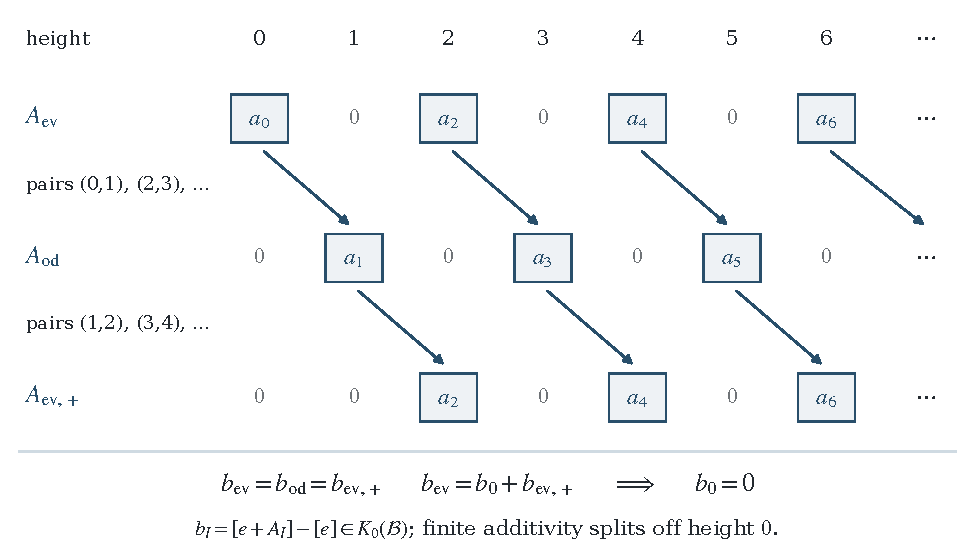
\includegraphics[width=\linewidth]{figures/parity-cancellation.pdf}
  \caption{Height supports of three bounded operator families. Each
  arrow represents the rotation in \eqref{eq:model-pair-rotation}
  followed by rescaling from $a_i$ to $a_{i+1}$. The disjoint pairs give
  the two homotopies. Finite additivity splits off the root family.
  Ellipses describe the supports of actual operators in $\mathcal B$;
  they do not denote an infinite sum of $K$-classes. A zero entry is a
  zero compact difference; the full projection retains its scalar part.}
  \label{fig:parity-cancellation}
\end{figure}

\subsection{The physical root and a supported projection homotopy}

Let $J_{0,\nu}\colon e_{\nu0}^{\mathrm{car}}\mathscr L_\nu
\to\mathscr K_\nu$ be inclusion in its zeroth summand.  If $n_0^B$ is the
number of surviving $\mathscr B_0$ vertices, define the finite operator
\begin{equation}\label{eq:physical-root-row}
 S_\nu=(n_0^B)^{-1/2}\sum_{v\in\mathscr B_0^{\mathrm{surv}}}
               R(t_v^{-1})T_0,
 \qquad v_\nu=S_\nu\chi_0\in A_\nu.
\end{equation}
All sums are finite.  The unrestricted norm of $S_\nu$ need not be uniformly
bounded.  For a source coset $h\HH$, however,
$R(t_v^{-1})\delta_{hf}=\delta_{hft_v}$, so
\eqref{eq:physical-root-row} is exactly the normalized constant transport
in \eqref{eq:assembly-cover-coordinates}, after spreading.  Thus on the
localized source space
\[
 v_\nu=\mathcal J\mathcal I_\nu J_{0,\nu}\chi_0.
\]
Lemma~\ref{lem:assembly-synthesis}, or just its single-height estimate,
gives
\begin{equation}\label{eq:root-row-approximation}
 \|v_\nu-V_\nu J_{0,\nu}\chi_0\|
       \le C_\nu2^{-344.5H_{0,\nu}}\longrightarrow0.
\end{equation}
In particular the $v_\nu$ form a uniformly bounded sequence, because
$\|V_\nu\|\le1$ and $\|\chi_0\|\le1$.  The factor $n_0^B$ has been
accounted for by the multiplicity estimate, rather than suppressed by
assuming that untrimmed sheet summation is an isometry.

Let $a_\nu^{\mathrm{phys}}=a_0(R(z),R(x))$ and let
$p_\nu^{\mathrm{phys}}=e+a_\nu^{\mathrm{phys}}$.
These are fixed-size matrices and the latter are exact projections in
$M_m(A_\nu)$.  Write $a^{\mathrm{phys}}=[(a_\nu^{\mathrm{phys}})]$ and
$v=[(v_\nu)]$ in the reduced quotient, tensoring $v$ with $I_m$ when it
acts on Bott matrices.  The cutoff is real, supported inside the controlled
source carrier, and is one on $\supp a_\nu^{\mathrm{phys}}$.  Equations
\eqref{eq:model-map-near-isometry} and
\eqref{eq:root-row-approximation} imply
\begin{equation}\label{eq:root-supported-isometry}
 v^*v a^{\mathrm{phys}}=a^{\mathrm{phys}}
       =a^{\mathrm{phys}}v^*v,
 \qquad
 \Theta(A_0)=v a^{\mathrm{phys}}v^*.
\end{equation}
For example $v_\nu^*v_\nu-\chi_0^2$ is norm null after restricting to
the cutoff's carrier, and multiplication by $a_\nu^{\mathrm{phys}}$
removes both cutoffs.  The second equality follows by multiplying
\eqref{eq:root-row-approximation} on both sides of the compact difference.
This argument uses a cutoff supported in the larger controlled carrier;
merely asking that a cutoff equal one on the smaller Bott support would not
by itself control its remaining norm.

\begin{lemma}[Supported Bott transport]\label{lem:supported-bott-rotation}
Let $B$ be a $C^*$-algebra, $e\in M_m(\C)$ a projection, and
$a=a^*\in M_m(B)$ such that $e+a$ is a projection in $M_m(B^+)$.
Suppose $v\in B$ is bounded, acts as $v\otimes I_m$ on the matrix factor,
and satisfies $v^*va=a$.  Then
\[
 [e+a]-[e]=[e+vav^*]-[e]\quad\hbox{in }K_0(B).
\]
No contraction assumption on $v$ or identity projection for a carrier is
needed.
\end{lemma}

\begin{proof}
The adjoint relation is $av^*v=a$.  Put $c=\cos t$, $s=\sin t$ and
\begin{equation}\label{eq:supported-bott-path}
 P_t=\begin{pmatrix}
 e+c^2a&cs\,av^*\\cs\,va&e+s^2vav^*
 \end{pmatrix},\qquad 0\le t\le\pi/2.
\end{equation}
It is self-adjoint.  With $W_t=(cI_m,sv)^T$ and
$E_{\mathrm{sc}}=\operatorname{diag}(e,e)$, this is
$E_{\mathrm{sc}}+W_taW_t^*$.  The scalar-factor assumption gives
$E_{\mathrm{sc}}W_t=W_te$.  Moreover
$aW_t^*W_ta=a^2$ and $ea+ae+a^2=a$.  Multiplication now gives
$P_t^2=P_t$.  The endpoints are
$\operatorname{diag}(e+a,e)$ and
$\operatorname{diag}(e,e+vav^*)$, proving the equality after one
fixed stabilization.  All nonscalar entries belong to $M_{2m}(B)$ and the
path is norm continuous.  Its modulus depends only on $\|a\|$ and
$\|v\|$.  In particular it is uniform for bounded coordinate sequences.
\end{proof}

Apply Lemma~\ref{lem:supported-bott-rotation} to
\eqref{eq:root-supported-isometry}.  By
\eqref{eq:model-root-zero} and the homomorphism $\Theta^+$,
\begin{equation}\label{eq:physical-bott-quotient-zero}
 [(p_\nu^{\mathrm{phys}})]-[e]=0
       \quad\hbox{in }K_0(\mathcal Q_r).
\end{equation}
The size in \eqref{eq:supported-bott-path} is $2m$, independently of the
number of transports, graph layers, sheets, or construction index.

\subsection{From the quotient to one finitely generated group}

The remaining two steps recover finite witnesses.  First, equality in the
norm sequence quotient gives equality at every sufficiently late
coordinate.  Then the group elements needed to approximate one such
witness generate the required subgroup.  These are concrete forms of
projection stability and continuity in $C^*$-algebra $K$-theory
\cite[Sections~4.5 and~5.2, Theorem~5.6.1]{Blackadar98}; we give the
witness constructions to keep their finite matrix sizes explicit.

\begin{lemma}[Eventual coordinate equality]\label{lem:eventual-coordinate-equality}
Let $B_\nu$ be unital $C^*$-algebras and let
$P_\nu,Q_\nu\in M_m(B_\nu)$ be projections in a fixed size.
If their classes agree in
$K_0((\prod B_\nu)/(\bigoplus B_\nu))$, then
$[P_\nu]=[Q_\nu]$ in $K_0(B_\nu)$ for all sufficiently large $\nu$.
\end{lemma}

\begin{proof}
The definition of $K_0$ supplies a projection $R$ in a finite matrix algebra
over the quotient and, after finite zero padding, a partial isometry $w$
with
\[
 w^*w=P\oplus R=:E,\qquad ww^*=Q\oplus R=:F.
\]
Lift $R$ to a bounded self-adjoint sequence $r_\nu$.  Its idempotence defect
tends to zero.  On a tail its spectrum avoids $1/2$, and spectral cutting
gives projections $R_\nu$ with $\|R_\nu-r_\nu\|\to0$.  Form the
corresponding $E_\nu,F_\nu$ and lift $w$ to a bounded sequence $b_\nu$.
Set $z_\nu=F_\nu b_\nu E_\nu$.  Then
\[
 \|z_\nu^*z_\nu-E_\nu\|\to0,
 \qquad\|z_\nu z_\nu^*-F_\nu\|\to0.
\]
For large $\nu$ these products are invertible in the respective corners.
The element
$z_\nu(z_\nu^*z_\nu)^{-1/2}$ is a partial isometry with initial
projection $E_\nu$ and final projection $F_\nu$; the latter assertion uses
invertibility in the $F_\nu$ corner.  Thus
$[P_\nu]+[R_\nu]=[Q_\nu]+[R_\nu]$, and cancellation in $K_0(B_\nu)$
proves the result.  Every stabilization used is finite and fixed after the
quotient witness has been chosen.
\end{proof}

\begin{proposition}[Reduced Bott vanishing]\label{prop:reduced-bott-vanishing}
For all sufficiently large $\nu$ in the chosen compatible sequence, the image
of the rank-zero Bott generator of $K_0(\Cr(\langle z,x\rangle))$ is zero integrally in
$K_0(\Cr(\Gamma_\nu))$.
\end{proposition}

\begin{proof}
Apply Lemma~\ref{lem:eventual-coordinate-equality} to
\eqref{eq:physical-bott-quotient-zero}.  At every coordinate
\eqref{eq:physical-bott-profile} identifies the difference with the physical
torus Bott generator.  Equation~\eqref{eq:right-left-regular} transfers the
equality to the usual left reduced algebra without changing the subgroup
elements or their functional-calculus projections.
\end{proof}

\begin{lemma}[A finite witness lies in a finitely generated subgroup]
\label{lem:finite-subgroup-witness}
Let $H\le\Gamma$ be finitely generated, and let $P,Q$ be fixed finite matrix
projections over $\Cr(H)$.  If their images have equal $K_0$ classes over
$\Cr(\Gamma)$, then some finitely generated subgroup $\Ginj$ with
$H\le \Ginj\le\Gamma$ already has $[P]=[Q]$ in $K_0(\Cr(\Ginj))$.
\end{lemma}

\begin{proof}
Choose one finite stabilization projection and a partial isometry witnessing
the equality over $\Cr(\Gamma)$.  Approximate their finitely many entries
by group polynomials, using self-adjoint approximations for the projection.
Adjoin all group elements in these finite supports to generators of $H$;
they generate a finitely generated subgroup $\Ginj$.  The reduced inclusion
$\Cr(\Ginj)\to\Cr(\Gamma)$ is isometric, since restriction of the regular
representation of $\Gamma$ to $\Ginj$ is a direct sum of regular representations
of $\Ginj$.  Thus the required small projection and partial-isometry defects have
the same bounds in $\Cr(\Ginj)$.  Spectral cutting gives the stabilizing
projection in $\Cr(\Ginj)$; compressing the approximate partial isometry to
the two corners and polar-normalizing it gives an exact witness there, just
as in Lemma~\ref{lem:eventual-coordinate-equality}.  Functional calculus
stays inside $\Cr(\Ginj)$.  The original projections $P,Q$ were retained
exactly throughout.
\end{proof}
